% !TEX encoding = UTF-8 Unicode
\documentclass[a4paper,12pt]{article}
 \usepackage[T1]{fontenc}
 \usepackage[utf8]{inputenc}
 \usepackage[magyar]{babel}
 \usepackage{graphicx}
 \usepackage{gensymb}
 \usepackage{float}
 \usepackage{mhchem}
 \usepackage{amsmath}
 \usepackage{amssymb}
 \usepackage{bm}
 \usepackage{geometry}
\geometry{a4paper,
		     tmargin = 35mm, 
		     lmargin = 25mm,
		     rmargin = 30mm,
		     bmargin = 30mm}

 \usepackage{graphicx}
\usepackage{fixltx2e}
\usepackage{multirow}
\usepackage{hyperref}
\usepackage{braket}
\usepackage{indentfirst}
%\usepackage[dvips]{graphicx}
%\usepackage{epstopdf}
\usepackage{float}
\usepackage{caption}
\usepackage{subcaption}
 \frenchspacing
 
 \interfootnotelinepenalty=10000
 
 \pagestyle{plain}
 
 \begin{document}
 
\begin{titlepage}
	\centering
	
\includegraphics[width=0.55\textwidth]{elte.png}\par\vspace{1cm}
	{\scshape\LARGE Korszerű vizsgálati módszerek laboratórium \par}
	
	\vspace{1cm}
	{\huge\bfseries Az atommag mágneses momentumának mérése\par}
	\vspace{1cm}
	{\Large\itshape Katona Dávid\par}
	\vspace{1cm}
	{\itshape Mérőtársak: Máthé Marcell, Olar Alex\par}
	\vspace{0.5cm}
	{\scshape Mérés dátuma: 2018. 03. 22.\par}


	\vfill

% Bottom of the page
	{\large  2018. 03. 23.\par}
\end{titlepage}


\tableofcontents

\newpage

\section{A mérés célja}
A mérés célja a proton giromágneses faktorának meghatározása, valamint a $^{19}$F mag és a proton g-faktor-arányának mérése.

\section{Bevezetés}
\subsection{Elméleti háttér}

Az protonok, neutronok spinjük révén mágneses momentummal rendelkeznek, melynek következtében egyes atommagok is eredő mágneses momentummal bírnak. A Zeeman-effektus révén külső mágneses térben a spin $z$ ($\vec{B_0}$ irányú) komponense szerint felhasad, a felhasadás utáni energiaszinteket írja le \aref{eq:zeeman}. egyenlet. A $\gamma$ a giromágneses arányossági tényező, $\mu_N$ a magmagneton, $m_N$ a nukleon tömege, $e$ az elemi töltés, $g$ pedig az ún. g-faktor.

\begin{equation}
	E = -\hat{\vec{\mu}}\vec{B_0} = -\gamma \hat{\vec{J}}\vec{B_0}=-\gamma \hat{J_z}B_0 =: g\frac{\hbar e}{2m_N}m_j B_0=:g\mu_Nm_jB_0
	\label{eq:zeeman}
\end{equation}

A fehasadás miatt az átmenet megfelelő frekveciájú fotonnal gerjeszthető, kihasználva, hogy a foton energiája $E=h \nu$. Ez $B_0\simeq 1T$ környékén rádiófrekvenciás tartományba esik. A mérés során ezt a frekvenciát határozzuk meg a minták esetében több különböző $B_0$ érték mellett, melyből számolható a g-faktor értéke.

\subsection{A mérési összeállítás}

A mérés során a mintát külső mágneses térbe helyezzük, melyet elektromágnessel hozunk létre. Az elektromágnes két tekercset tartalmaz: az elsőn áramgenerátorral\footnote{Az állandó áramerősség miatt nem kell számolni a tekercs melegedéséből eredő ellenállásváltozással.} állandó áramerősséget folyatunk át, a másikkal ezt a konstans $B_0$ teret moduláljuk $25Hz$ frekvenciával $1-2\%$ mértékben. Erre azért van szükség, hogy egy $B$ tartományon mérve, az abszorpció mértékét oszcilloszkópon megjelenítve a moduláló jel ($\sim (B-B_0)$) függvényében a rezonancia csúcsként fog megjelenni egy adott ponton az oszcilloszkóp kijelzőjén.

A gerjesztést egy tekerccsel végezzük. Ugyanezt a tekercset használjuk az abszorpció mérésére is, mivel a tekercs oszcillátor-kapcsolásba van kötve, így az abszorpciót az oszcillátor amplitúdó-csökkenése mutatja. Ezt az oszcilloszkóp függőleges tengelyén megjelenítva detektáljuk az abszorpciót. 

A kívánt paraméterek meghatározásához szükség van a frekvencia és a mágneses térerősség pontos mérésére. A frekvenciamérést egy jelgenerátorra kötött antennával végezzük. A jelgenerátor kijelzőéről nagyobb pontossággal leolvasható az általa generált jel frekvenciája. Amikor az antennára kötött jel frekvenciája és a gerjesztőfrekvencia igen közel esik egymáshoz lebegés jön létre, melyet az oszcilloszkópon látunk. Ezzel meghatározható a gerjesztési frekvencia.

A mágneses tér mérésére ballisztikus galvanométert használunk. Ezt a mágneses térbe helyezve, majd onnan határozott mozdulattal kirántva a fluxusváltozásból határozza meg a mágneses tér erősségét. A fluxusváltozás feszültséget generál, amely áramot hoz létre, ezt pedig időben kiintegrálva (töltésmennyiség) a mágneses tér erősségéval arányos jelet kapunk. A kalibrációt felhasználva így meghatározható $B_0$ nagysága.

\section{Mérési eredmények}

\subsection{A proton g-faktorának meghatározása}

Vízminta (CuSO$_4$-oldat) esetén megmértük több különböző mágneses térben a frekvenciát. Az adatokat \aref{tab:proton_all}.táblázat tartalmazza.

\begin{table}[h]
	\begin{center}
	\begin{tabular}{|c|c|c|c|}
		\hline
		\textbf{Frekvencia [MHz]} & \textbf{Áramgenerátor állása} & \textbf{Áramerősség [A]} & \textbf{Galvanométer értéke} \\
		\hline \hline
		8.496	& 782	&2.42	&60.5 \\  
		\hline
		8.325	&766		&2.37	&60 \\ \hline
		\textit{7.705}	&\textit{685}		&\textit{2.12}	&\textit{55.5} \\ \hline
		7.285	&626.5	&1.94	&52.5 \\ \hline
		7.155	&610		&1.89	&51.5 \\ \hline
		\textit{6.754}	&\textit{623.5}	&\textit{1.93}	&\textit{48.5}	\\ \hline
		6.167	&566.0	&1.74	&44 \\	 \hline
		5.641	&514.0	&1.57	&41 \\ \hline
		\textit{5.087}	&\textit{445.5}	&\textit{1.38}	&\textit{36.5}	 \\ \hline
		4.515	&373.0	&1.15	&33	\\  \hline
		4.064	&324.0	&1.00	&29.5	\\ \hline
		\textit{3.675}	&\textit{284.5}	&\textit{0.87}	&\textit{28.5}	 \\ \hline
	\end{tabular}
	\end{center}
	\caption{Mérési adatok a víz esetében. A kiértékeléshez általam használt adatok dőlttel vannak jelölve.}
	\label{tab:proton_all}
\end{table}

\subsubsection{Hibaforrások}
A galvanométer állásából számolható a mágneses indukció nagysága a kalibrációt adatot felhasználva, miszerint a galvanométer egy osztása $3.35\pm0.1 mT$-nak felel meg. Elviekben lehetséges lenne az áramerősségből, illetve a még pontosabban meghatározható áramgenerátor állásából kalibrációs egyenest használva B értékének kisebb hibájú meghatározása, de mivel a mérési pontok felvétele során az áramerősség nem monoton változott időben, emiatt a vasmag felmágneseződése miatt hiszterézis lépett fel, mely \aref{fig:hist}. ábra alapján egyértelműen látható.

\begin{figure}[h]
\centering
    \begin{minipage}{.99\textwidth}
        \centering
        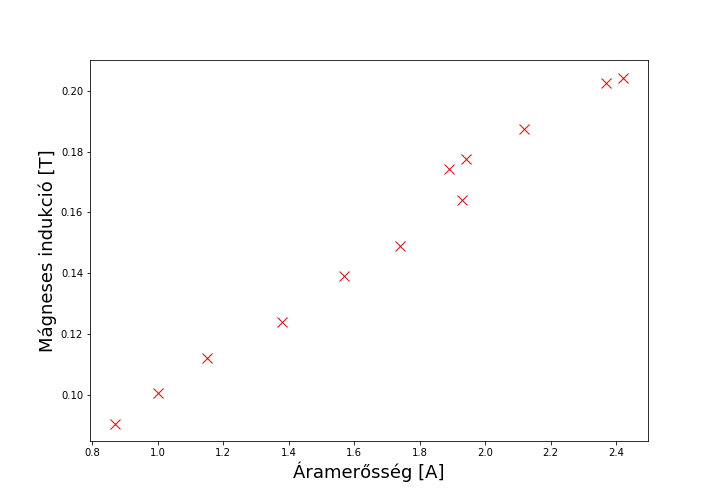
\includegraphics[width=1.\linewidth]{hiszterezis.png}
    \end{minipage}
    \caption{Mért mágneses tér az áramerősség függvényében. Az ábrán megfigyelhető a hiszterézis jelensége.}
    \label{fig:hist}
\end{figure}

A $B_0$ mérése során szisztematikus hibaforrás a galvanométer kalibrálási bizonytalansága. Statisztikus hibaként jelenik meg a leolvasás pontossága, amely ismételt leolvasási kísérletek alapján $\pm 0.5$ egység. Ezen túl hibaforrás a galvanométer-mérőfej, valamint a minta eltérő pozíciója a tér inhomogenitása miatt. Ennek becsléséhez hosszirányban megnéztem a tér inhomogenitását, azaz, a minta jelének eltolódását\footnote{Az oszcilloszkóp kijelzőjén való eltolódás alapján határoztuk meg. Ehhez előzőleg frekvenciaméréssel meghatároztuk, hogy 1 beosztás az oszcilloszkóp kijelzőjén $\nu=5.5MHz$-nél $0.30\%$ eltérésnek felel meg. Mivel $B\sim \nu$, ezért ez $B$-nek is ekkora hibáját jelenti.} z tengely szerint (\ref{fig:z_inhom}. ábra). A másik két irányban a mérőtársaim határozták meg az inhomogenitás mértékét, azonban azon irányokban inkább kisebbnek mondható. Ez alapján az inhomogenitásból eredő hibát $\delta B_\text{inhom} \simeq 0.15\%$-ra becsülöm, mivel kb. $0.8cm$-es $z$ irányú tartományon ennél kisebb az ingadozása $B$-nek. Adott nagyságú mágneses térben az összes paraméter ($B$, $\nu$, beállítások értékei) lemérése 1-2 percet vett igénybe, ez alatt a mágneses tér nem teljesen állandó. Az ebből eredő hiba $0.18\%$ volt 2 perc alatt\footnote{Meghatározását ugyanúgy frekvenciamérésre vezettük vissza, mint az inhomogenitásét.}. Az abszorpciós jel középre állításának hibája $< 0.03\%$.

\begin{figure}[h]
\centering
    \begin{minipage}{.99\textwidth}
        \centering
        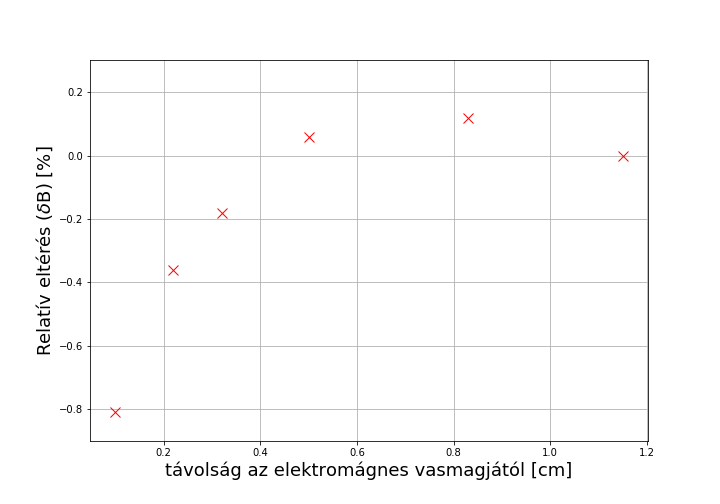
\includegraphics[width=1.\linewidth]{inhom.png}
    \end{minipage}
    \caption{A mágneses tér ihomogenitása z irányban.}
    \label{fig:z_inhom}
\end{figure}

A frekvenciamérés hibája három faktorból tevődik össze: i.) a leolvasás hibája ii.) a jelgenerátor frekvenciamérésének hibája iii.) a lebegés reprodukálhatóságának bizonytalansága. Az első mértéke $\pm0.0005MHz$, a másodikat csupán becsülni tudjuk, de a kvarcórák hibájából kiindulva $< 10^{-5}$, a reprodukálhatósági próbánál pedig a hiba kisebb a kijelzési pontosságnál. A frekvenciamérés hibája tehát jó közelítéssel $\pm0.0005MHz$.

\subsubsection{A proton g-faktorának értéke}

A mért adatok alapján számolt frekvenciákat és $B_0$ értékeket mutatja \aref{tab:szamolt}. táblázat. Mivel az időmérés hibája jóval kisebb, ezért a frekvencia függvényében ábrázolva a $B_0$ értékeket origón átmenő egyenest\footnote{Ellenőrzésképp konstans taggal rendelkező egyenest illesztve a konstans paraméter értéke ($-0.16\pm7.2)\cdot10^{-4}T$, tehát valóban nullán átmenő egyenest kapunk így is.} illesztettem (\ref{fig:BF}. ábra), melynek meredeksége: $m=(2.409\pm0.0025)\cdot10^{-8}Ts$. Ebből számolható $g_p = 5.45\pm0.17$, ahol az egyenesillesztés hibájához négyzetesen hozzáadtam a galvanométer kalibrációs hibáját is. Ez az érték hibahatáron belül közelíti az irodalmi értéket ($g= 5.585$).
\begin{table}[h]
	\begin{center}
	\begin{tabular}{|c|c|}
		\hline
		Frekvencia [MHz] & B [mT] \\ \hline \hline 

		$ 7.705\pm 0.0005 $&$185.9\pm 1.7 $  \\ \hline 

		$ 6.754\pm 0.0005 $&$162.5\pm 1.7 $  \\ \hline 

		$ 5.087\pm 0.0005 $&$122.3\pm 1.7 $  \\ \hline 

		$ 3.675\pm 0.0005 $&$88.8\pm 1.7 $  \\ \hline 

	\end{tabular}
	\end{center}
	\caption{Számolt frekvencia és $B_0$ értékek }
	\label{tab:szamolt}
\end{table}

\begin{figure}[h]
\centering
    \begin{minipage}{1\textwidth}
        \centering
        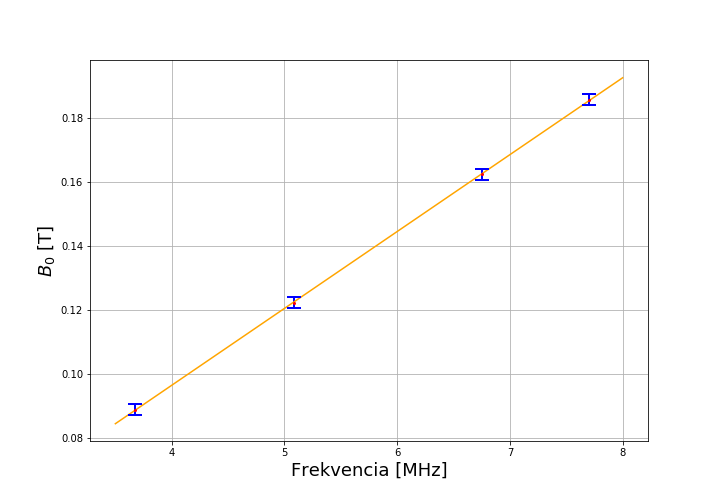
\includegraphics[width=1\linewidth]{BF.png}
    \end{minipage}
    \caption{$B_0$ a gerjesztőfrekvencia függvényében vízmintánál}
    \label{fig:BF}
\end{figure}

\subsection{Fluor és proton g-faktor-arányának mérése}
\subsubsection{Hibaforrások}
A fluor g-faktorának (relatív) meghatározásához adott $B_0$ térerősség mellett egymás után meghatároztuk a proton és a fluor abszorpciócsúcsához tartozó frekvenciát. A mérés előnye, hogy a mágneses tér mérésének hibája kiesik. Itt csak az 1-2 perces mérési időből származó $0.18\%$-os eltéréssel kell számolnunk, ami a mágneses tér időbeli ingazdozása. Mivel csak a mintát cseréltem ki, nem pedig az egész mérőtekercset távolítottuk el mérésről mérésre, ezért a hely hibája igen kicsi, $<2mm$, ami alapján a $B_0$ inhomogenitásból eredő hibája $<0.06\%$. Összességében tehát $\delta B_0 \simeq 0.19\%$.

A frekvenciamérés hibája adódik a leolvasás pontatlanságából ($\pm0.0005MHz$), valamint a szélesebb és laposabb flour-csúcs beállításának bizonytalanságából. Ez utóbbi az oszciloszkópon $\pm0.2$ osztásnak becsülöm, ami $\pm 0.0034MHz$-nek felel meg. Proton esetében ugyanez az érték $\pm 0.001MHz$, mivel annak jóval élesebb a csúcsa.

Az aránymeghatározást tehát itt a mágneses tér időbeli inhomogenitásból eredő hibája dominálja, azonban itt a mérés teljes bizonytalansága csupán $0.20\%$, mivel közvetlen nem kell mérni a $B_0$ értékét.

\subsubsection{A fluor g-faktora}
A mért eredményeket tartalmazza \aref{tab:fluor}. táblázat. Mivel a hibák közel azonosak, az arányok atlagát véve meghatározható $\frac{g_F}{g_p} = 0.9404 \pm 0.0019$. Az irodalmi érték $0.9409(3)$, tehát hibahatáron belül megkaptuk.

\begin{table}[h]
	\begin{center}
	\begin{tabular}{|c|c|}
		\hline
		proton  [MHz] & fluor [MHz]\\ \hline \hline 

		$4.996\pm 0.001$	&$4.697\pm0.003$  \\ \hline 

		$7.150\pm 0.001$	&$6.726\pm0.003$  \\ \hline 

	\end{tabular}
	\end{center}
	\caption{A fluor és a proton adott $B_0$ melletti rezonanciafrekvenciája. }
	\label{tab:fluor}
\end{table}


\end{document}
